% This file was created by matlab2tikz.
%
%The latest updates can be retrieved from
%  http://www.mathworks.com/matlabcentral/fileexchange/22022-matlab2tikz-matlab2tikz
%where you can also make suggestions and rate matlab2tikz.
%
\definecolor{mycolor1}{rgb}{0.00000,0.44700,0.74100}%
\definecolor{mycolor2}{rgb}{0.85000,0.32500,0.09800}%
%
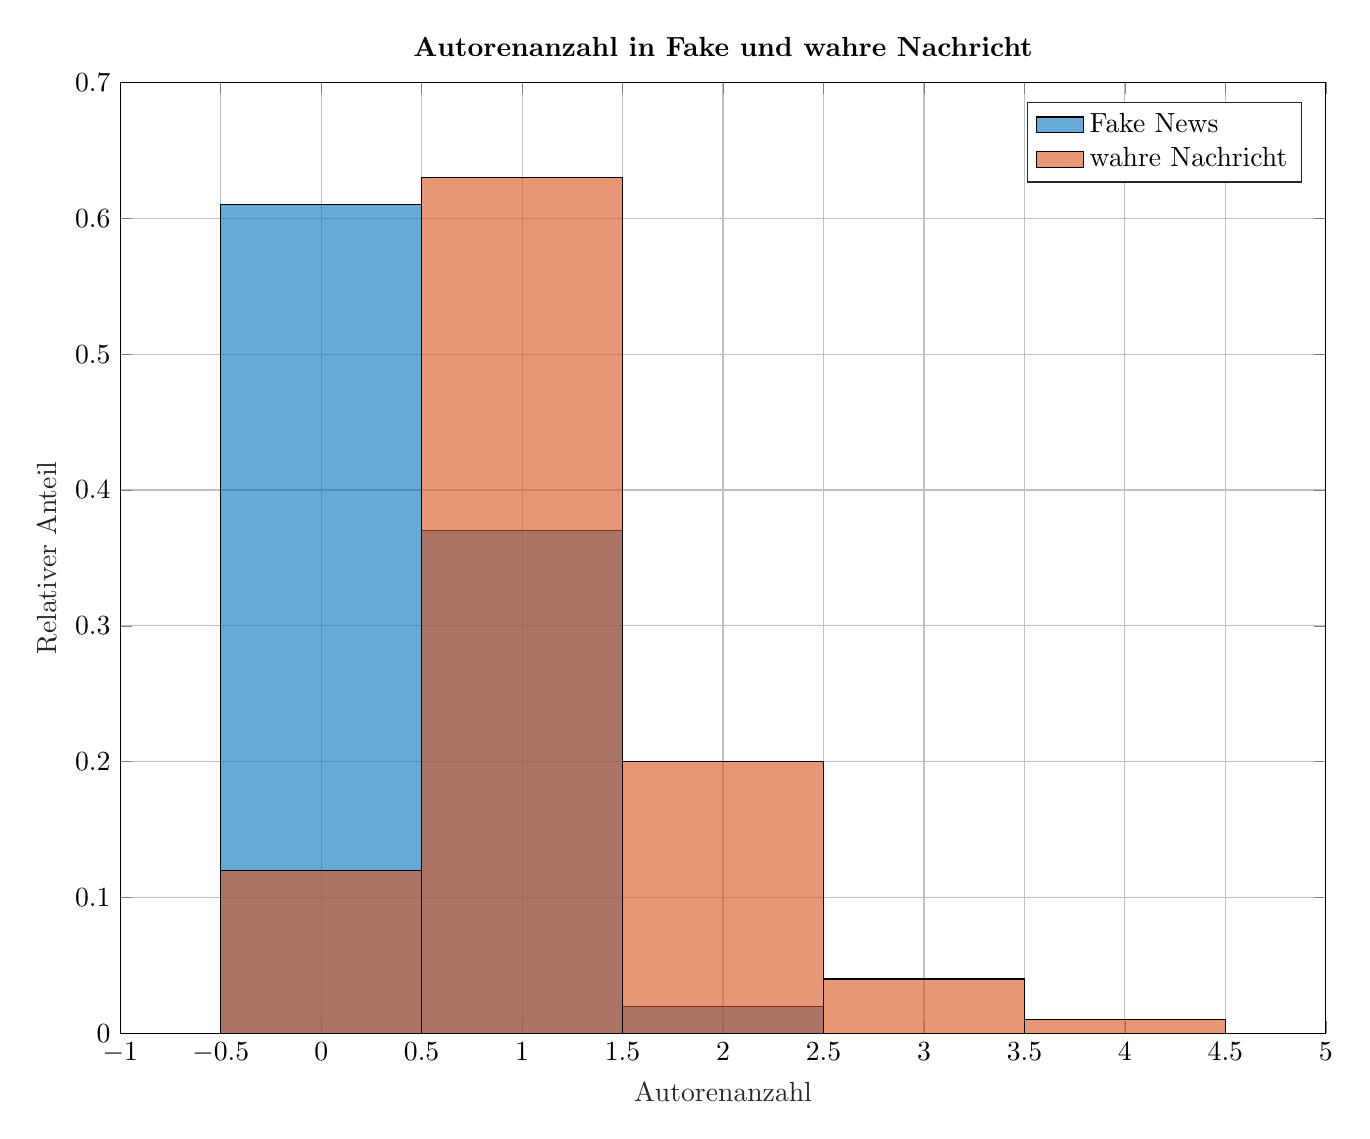
\begin{tikzpicture}

\begin{axis}[%
width=6.028in,
height=4.754in,
at={(1.011in,0.642in)},
scale only axis,
xmin=-1,
xmax=5,
xlabel style={font=\color{white!15!black}},
xlabel={Autorenanzahl},
ymin=0,
ymax=0.7,
ylabel style={font=\color{white!15!black}},
ylabel={Relativer Anteil},
axis background/.style={fill=white},
title style={font=\bfseries},
title={Autorenanzahl in Fake und wahre Nachricht},
xmajorgrids,
ymajorgrids,
legend style={legend cell align=left, align=left, draw=white!15!black}
]
\addplot[ybar interval, fill=mycolor1, fill opacity=0.6, draw=black, area legend] table[row sep=crcr] {%
x	y\\
-0.5	0.61\\
0.5	0.37\\
1.5	0.02\\
2.5	0.02\\
};
\addlegendentry{Fake News}

\addplot[ybar interval, fill=mycolor2, fill opacity=0.6, draw=black, area legend] table[row sep=crcr] {%
x	y\\
-0.5	0.12\\
0.5	0.63\\
1.5	0.2\\
2.5	0.04\\
3.5	0.01\\
4.5	0.01\\
};
\addlegendentry{wahre Nachricht}

\end{axis}
\end{tikzpicture}%